\documentclass[11pt]{article}
\usepackage[margin=1in]{geometry}
\usepackage{amsmath,booktabs,graphicx,hyperref}
\title{Quality-conditioned ranking for low-dose CT image quality assessment}
\author{M. Samiul Hasnat\\\small Affiliation and correspondence details to be confirmed}
\date{25 November 2026}
\begin{document}
\maketitle
\noindent\textbf{Internal research draft.} Author information, institutional declarations and the final journal format require author review. This document records exploratory experiments; it does not claim clinical validation or state-of-the-art performance.
\section*{Abstract}
High correlation on a small computed tomography (CT) image-quality benchmark need not imply agreement with expert preferences under domain shift. We study a quality-conditioned blur-ranking constraint that applies a synthetic preference assumption only to highly rated training images, without assigning scores to altered images. Nine scalar and ordinal configurations using EfficientNet-B0 or ResNet-18 are evaluated across three seeds, giving 27 models. Development uses inferred image-similarity groups; evaluation uses the released 300-image low-dose CT test collection and 1,666 independently expert-rated cone-beam CT phantom images. The scalar EfficientNet baseline achieves aggregate correlation $2.7200\pm0.0133$; adding the mild conditional constraint gives $2.7197\pm0.0040$, without establishing statistical equivalence. External signed Spearman correlation changes from $-0.142$ to $0.348$, and reconstruction-pair agreement from 42.5\% to 74.5\%. The corresponding unconditional constraint gives 49.3\% pair agreement. However, an ordinal mild-blur model eliminates synthetic blur score increases yet has external correlation $-0.097$, and ResNet-18 transfer remains poor. Removing the quality gate from a stronger ordinal constraint produces similar external performance. These exploratory controls distinguish benchmark accuracy, synthetic consistency and expert-rated transfer. Quality conditioning helps in one scalar configuration but is not a universal solution; two phantoms, substantial seed variation, adaptive follow-ups and unverified development patient identities limit generalization claims.
\section{Introduction}
Reducing CT dose can increase noise and reconstruction artifacts, while postprocessing can suppress noise at the cost of fine structure. A useful image-quality predictor must therefore reflect more than a single property such as smoothness. The LDCT perceptual quality challenge established a common abdominal CT benchmark with radiologist mean opinion scores (MOS), permitting reproducible evaluation of no-reference methods \cite{challenge}. Its winning approach combined convolutional and transformer predictors with ordinal scoring losses \cite{winner,rps}. Subsequent approaches include medical vision-language representations and reading-inspired networks \cite{medsiglip,clinreadnet}.

High benchmark correlation is valuable, but its interpretation depends on the data, score representation and evaluation history. Recent author comparisons show that a conventional EfficientNet-B0 at sufficiently high resolution is competitive with substantially larger models \cite{medsiglipcode}. A recent measurement-aware model also highlights the difficulty of distinguishing noise suppression from excessive smoothing \cite{measurement}. These findings motivate a focused question: can a small model be trained to respond more consistently to structural degradation without requiring an additional inference network?

We investigate a conditional degradation-ranking term attached to compact scalar and ordinal predictors. Its underlying assumption is deliberately limited: for relatively highly rated training images, an additional blur should not receive a higher predicted score. We do not assume that every blurred noisy image has lower diagnostic quality. The threshold makes this assumption conditional on observed training quality, but it remains a heuristic that requires evaluation against expert preferences. We therefore pair controlled synthetic probes with an independent expert-rated CBCT phantom dataset \cite{cbctpaper,cbctdata}.

The study compares nine configurations across three seeds, including scalar and ordinal predictors, two blur strengths, matched unconditional constraints, and a ResNet-18 portability control. It evaluates transfer using human ratings rather than algorithm-derived labels and retains unsuccessful outcomes. EfficientNet, ordinal losses and smoothing-bias diagnosis are established ideas. The scientific question concerns the effects and limits of the conditional constraint; the architecture alone is not presented as novel.
Learning quality rankings from synthetic distortions has substantial prior art. RankIQA uses automatically generated distortion rankings for pretraining \cite{rankiqa}, and distortion-guided learning has also been studied for opinion-unaware low-dose CT IQA \cite{distortionct}. Our supervised study uses training MOS to restrict a blur preference assumption and evaluates the resulting behavior against independent expert-rated reconstructions. It does not claim to introduce synthetic degradation ranking or to outperform opinion-unaware methods under their different supervision setting.

\noindent\textbf{Keywords:} computed tomography; image quality assessment; degradation ranking; domain transfer; phantom validation
\section{Materials and methods}
\subsection{Compact scalar and ordinal predictors}
The principal configurations use an EfficientNet-B0 backbone \cite{efficientnet} initialized with the offline \path{timm/efficientnet_b0.ra_in1k} weights. Normalized grayscale images are clipped to $[0,1]$, resized to $448\times448$ with floating-point bicubic interpolation, replicated over three channels and normalized using the ImageNet channel statistics. The portability control uses ImageNet-pretrained ResNet-18 with the same input pipeline and scalar head. Augmentation comprises horizontal and vertical flips. Noise, contrast changes and crops are not assigned unchanged MOS labels.

The scalar baseline pools backbone features and applies a 256-unit GELU head with dropout 0.1, followed by a bounded score $4\,\mathrm{sigmoid}(z)$. The ordinal configuration replaces the final scalar output with 21 logits over $b_k=0.2k$, $k=0,\ldots,20$. Its score is the expectation
\begin{equation}
 q_\theta(x)=\sum_{k=0}^{20}b_k p_{\theta,k}(x),\qquad
 p_\theta(x)=\mathrm{softmax}(z_\theta(x)).
\end{equation}
The ordinal probabilities encode a training target constructed from the MOS, not an observed distribution of individual reader votes and not a calibrated clinical uncertainty estimate.

\subsection{Supervised objective}
For an MOS between adjacent grid points, the target distribution places linearly interpolated mass on those points. The ordinal loss is
\begin{equation}
 \mathcal L_{\mathrm{sup}}=\mathcal L_{\mathrm{MSE}}
 +0.5\mathcal L_{\mathrm{rank}}+\mathcal L_{\mathrm{CDF}},
\end{equation}
where $\mathcal L_{\mathrm{CDF}}$ averages squared differences between predicted and target cumulative probabilities over the 20 nonconstant thresholds. This is an ordinal scoring objective motivated by ranked probability scores \cite{rps}. The scalar baseline uses the same MSE and ranking terms without the CDF term.

For consistency with the existing baseline, pairwise ranking uses margin 0.1 and averages the complete within-batch pair matrix, including diagonal and tied-target pairs. Those pairs contribute constants with zero prediction gradient. All configurations use batch size 32; the scale of this objective is not compared across different batch sizes.

\subsection{Quality-conditioned degradation ranking}
Let $B_\sigma$ denote Gaussian smoothing in normalized image space after resizing. For the training subset $H=\{i:y_i\geq3\}$, we define
\begin{equation}
 \mathcal L_{\mathrm{cond}}=\frac{1}{|H|}\sum_{i\in H}
 \max\{0,0.1-q_\theta(x_i)+q_\theta(B_\sigma(x_i))\}.
\end{equation}
The term is zero when a batch contains no eligible image. Training uses $\mathcal L_{\mathrm{sup}}+0.1\mathcal L_{\mathrm{cond}}$. Original and altered auxiliary predictions are computed with batch-normalization running statistics fixed and dropout disabled; gradients still flow through both scores. This prevents the extra synthetic forwards from updating running statistics. No MOS is assigned to the altered image. At inference, the model uses one backbone and its scalar or ordinal head; the constraint adds no image-processing branch.

An initial $\sigma=1.5$ arm was specified before inspecting the new arms' test results. Development probes then showed that highly rated images were more often rewarded after milder smoothing, and the initial auxiliary training loss was frequently zero. We retained the initial arm and declared a $\sigma=0.75$ follow-up with the same weight, threshold and margin. This adaptive development history is disclosed rather than treated as a preregistered comparison. Further exploratory controls apply the same mild constraint to the scalar head, repeat the scalar comparison using ResNet-18, and remove the quality gate (threshold 0) for scalar mild-blur and ordinal strong-blur constraints. These follow-ups were declared after initial external results were available. They do not use external labels to fit parameters, but their interpretation is exploratory. All nine arms and all seeds are reported; no externally selected configuration is treated as a new confirmatory result.
\begin{table}[ht]\centering\small
\caption{Declared configurations. Each uses three seeds. C denotes a constraint restricted to training MOS $\geq3$; U applies it to every training image. Gaussian $\sigma$ is measured at the 448-pixel input resolution.}
\begin{tabular}{lllr}\toprule Model & Backbone & Constraint & $\sigma$ \\ \midrule
Scalar & EfficientNet-B0 & None & -- \\
Ordinal & EfficientNet-B0 & None & -- \\
Ordinal + blur 1.5 & EfficientNet-B0 & C & 1.5 \\
Ordinal + blur 0.75 & EfficientNet-B0 & C & 0.75 \\
Scalar + conditional blur 0.75 & EfficientNet-B0 & C & 0.75 \\
Scalar + unconditional blur 0.75 & EfficientNet-B0 & U & 0.75 \\
ResNet-18 scalar & ResNet-18 & None & -- \\
ResNet-18 + conditional blur 0.75 & ResNet-18 & C & 0.75 \\
Ordinal + unconditional blur 1.5 & EfficientNet-B0 & U & 1.5 \\
\bottomrule\end{tabular}\label{tab:design}\end{table}
\subsection{Experimental design}
\subsection{LDCT development and test data}
The challenge separates training, validation and test data at the patient level \cite{challenge}. We use the released 1,000-image training collection for development and the separate released 300-image test collection for evaluation. The training files do not provide a verified patient mapping in the materials available to this study.

To reduce near-duplicate leakage during development, $64\times64$ normalized image thumbnails are grouped by connected components at correlation threshold 0.99955. This produces 99 inferred groups: 98 containing ten images and one containing twenty. A fixed group assignment gives 790 training and 210 validation images. These image-similarity groups are not patient identifiers; different groups may still belong to the same patient. The original filename-based 700/200/100 split was not used to support the new model-development claims.

The released test archive was obtained through the link in a public author repository \cite{medsiglipcode}. Its labels agree with a separately available public copy. Its SHA-256 and provenance are preserved in the research audit. Image-level identity with the organizers' original download has not been independently verified. The public test was used for earlier exploratory checkpoint evaluations before this study, so it is not an untouched confirmatory holdout. Models and constraint settings in the current study were developed using validation evidence, and all declared seeds are retained.

\subsection{Optimization and evaluation}
Each arm uses seeds 42, 123 and 456, AdamW with learning rate $10^{-4}$ and weight decay 0.01, a cosine schedule to $10^{-6}$, mixed-precision training, gradient clipping at 1 and a maximum of 100 epochs. Early stopping requires at least 20 epochs and 20 epochs without selection improvement. Checkpoints maximize the signed sum of validation correlations. The existing scalar runs select using four-decimal correlation components, whereas the new control arms use unrounded values; this small implementation difference is disclosed.

We report Pearson, Spearman and Kendall correlations, the challenge aggregate $A=|r|+|\rho|+|\tau_b|$, and MAE. All reported correlations are recomputed from the saved continuous predictions, without rounding individual correlation components. Predictions are neither rounded onto the MOS grid nor calibrated with test labels. Means and sample standard deviations across seeds describe training variation on one fixed test collection. They are not confidence intervals for a population of patients. Literature results are presented as context; differences in folds, ensembles, rounding and selection prevent unqualified ranking against published numbers.

\subsection{Synthetic development probes}
Every checkpoint is probed on all 210 validation images using Gaussian smoothing with $\sigma=0.75,1.5,2.5$, a box filter of width 5, and additive Gaussian noise with standard deviation 0.01 or 0.03 in normalized units. Noise is deterministically seeded per image. For the mild-constraint arm, the larger Gaussian settings and box filter are not used by its training constraint. We report predicted-score changes overall and within original MOS strata $y\geq3$ and $y\leq1$; there are 49 validation images in each of these strata. The probes do not provide new human quality labels.

\subsection{Independent phantom transfer}
CBCT-IQ contains acquisitions of thorax and pelvis anthropomorphic phantoms with expert overall and region-specific quality ratings \cite{cbctpaper,cbctdata}. We use the actual 1,666 rows of the released annotation file, independently verifying the archive and annotation checksums. All annotated rows are uniquely matched to an image, accounting for the published directory-order difference and the \texttt{VSMOOTH}/\texttt{VERYSMOOTH} naming difference. The NIfTI RAS voxel axes are mapped to axial image rows and columns from the image geometry, preserving the reference normalization. Initial stored-array evaluations were stopped after visual input checks revealed a rotated presentation; all models were rerun with the geometry correction. No orientation was selected by predictive performance. Model input clipping does not alter pixel values in the prepared external cases.

The primary external endpoint is signed Spearman correlation with human \texttt{OIQ\_MOS\_ZSCORE}, overall and separately by phantom anatomy. We do not use the algorithm-derived IQA-rating columns as reader labels and do not compare absolute errors across incompatible rating scales. A secondary endpoint measures agreement between model preferences and at least two of three readers for reconstruction pairs matched on anatomy, slice, kernel, voltage and pulse width. Ambiguous or tied reader pairs are counted separately, and model ties within $10^{-6}$ receive half credit. No ratings are fabricated for unannotated reference acquisitions. CBCT-IQ readers scored images with a reference visible, whereas the models receive only the test image; this differs from the LDCT annotation task. The published rubric confirms that larger reader scores indicate better quality.

Final external inference uses the original two GPUs and PyTorch 2.13 environment for all models. Local CPU runs with PyTorch 2.15 are retained as numerical checks; a 32-image comparison against the original GPU predictions showed a maximum absolute difference of approximately 0.0029 MOS units. Those environments are not treated as numerically identical. Source snapshots, full version records, model hashes and per-image outputs are retained. Paired external differences are summarized with 2,000 bootstrap resamples of 98 source-slice groups, stratified by anatomy (71 thorax, 27 pelvis), keeping all reconstructions of a selected source slice together. Each endpoint is averaged over the same three fixed seeds. Percentile intervals are conditional on these two physical phantoms; correlated slices and fixed seeds prevent interpreting them as patient- or site-population confidence intervals.
\section{Results}
\begin{table}[ht]\centering\small
\caption{Released LDCT test results, mean $\pm$ sample SD over three training seeds on one fixed test collection.}
\begin{tabular}{lrr}\toprule Model & Aggregate $\uparrow$ & MAE $\downarrow$ \\ \midrule
Scalar & $2.7200\pm0.0133$ & $0.3010\pm0.0021$ \\
Ordinal & $2.6931\pm0.0201$ & $0.2961\pm0.0276$ \\
Ordinal + blur 1.5 & $2.6912\pm0.0194$ & $0.2965\pm0.0260$ \\
Ordinal + blur 0.75 & $2.7016\pm0.0168$ & $0.2895\pm0.0234$ \\
Scalar + conditional blur 0.75 & $2.7197\pm0.0040$ & $0.3164\pm0.0327$ \\
Scalar + unconditional blur 0.75 & $2.7070\pm0.0139$ & $0.3261\pm0.0101$ \\
ResNet-18 scalar & $2.6256\pm0.0075$ & $0.4249\pm0.0522$ \\
ResNet-18 + conditional blur 0.75 & $2.6064\pm0.0371$ & $0.4043\pm0.0536$ \\
Ordinal + unconditional blur 1.5 & $2.6928\pm0.0236$ & $0.3084\pm0.0396$ \\
\bottomrule\end{tabular}\label{tab:ldct}\end{table}
\begin{table}[ht]\centering\small
\caption{External CBCT-IQ phantom transfer, mean $\pm$ seed SD. All models use fixed inference on 1,666 expert-annotated slices.}
\begin{tabular}{lrr}\toprule Model & Spearman $\uparrow$ & Pair agreement $\uparrow$ \\ \midrule
Scalar & $-0.142\pm0.253$ & $0.425\pm0.158$ \\
Ordinal & $-0.222\pm0.328$ & $0.376\pm0.213$ \\
Ordinal + blur 1.5 & $0.426\pm0.255$ & $0.737\pm0.144$ \\
Ordinal + blur 0.75 & $-0.097\pm0.215$ & $0.484\pm0.092$ \\
Scalar + conditional blur 0.75 & $0.348\pm0.307$ & $0.745\pm0.149$ \\
Scalar + unconditional blur 0.75 & $-0.075\pm0.485$ & $0.493\pm0.264$ \\
ResNet-18 scalar & $-0.603\pm0.130$ & $0.034\pm0.055$ \\
ResNet-18 + conditional blur 0.75 & $-0.470\pm0.116$ & $0.118\pm0.111$ \\
Ordinal + unconditional blur 1.5 & $0.391\pm0.063$ & $0.728\pm0.059$ \\
\bottomrule\end{tabular}\label{tab:external}\end{table}
\begin{table}[ht]\centering\small
\caption{External signed Spearman correlation by phantom anatomy, mean $\pm$ seed SD. The thorax and pelvis contain 1,207 and 459 annotated images, respectively.}
\begin{tabular}{lrr}\toprule Model & Thorax & Pelvis \\ \midrule
Scalar & $-0.045\pm0.386$ & $-0.273\pm0.677$ \\
Ordinal & $-0.096\pm0.433$ & $-0.630\pm0.309$ \\
Ordinal + blur 1.5 & $0.506\pm0.188$ & $0.196\pm0.672$ \\
Ordinal + blur 0.75 & $0.080\pm0.182$ & $-0.385\pm0.375$ \\
Scalar + conditional blur 0.75 & $0.552\pm0.199$ & $0.041\pm0.464$ \\
Scalar + unconditional blur 0.75 & $0.131\pm0.522$ & $-0.491\pm0.323$ \\
ResNet-18 scalar & $-0.822\pm0.060$ & $-0.719\pm0.214$ \\
ResNet-18 + conditional blur 0.75 & $-0.582\pm0.249$ & $-0.660\pm0.025$ \\
Ordinal + unconditional blur 1.5 & $0.568\pm0.067$ & $0.095\pm0.248$ \\
\bottomrule\end{tabular}\label{tab:anatomy}\end{table}

\subsection{Benchmark performance and efficiency}
The scalar compact model has the highest mean test aggregate among the original four compact arms. The ordinal head alone does not improve this metric. Mild conditional ranking improves the ordinal arm's mean aggregate from 2.6931 to 2.7016 and lowers its mean MAE, while the scalar model remains ahead in aggregate correlation. These observations do not establish superiority over current published methods or statistical equivalence to the scalar model. The scalar mild-constraint arm achieves aggregate 2.7197 with mean MAE 0.3164, compared with 2.7070 and 0.3261 after removing its quality gate. ResNet-18 achieves 2.6256 without the constraint and 2.6064 with it. These controls do not support a universal benchmark-accuracy gain from conditional ranking.

The scalar network has 4,335,741 parameters and the ordinal head increases this count by 5,140. An earlier aligned multi-scale transformer has 88,325,379 parameters and scores 2.5885 in a single exploratory run. That pipeline differs in several settings and is not a controlled architecture-only comparator. In one RTX 4090 benchmark, scalar compact forwards require 24.9 ms per batch of 32, compared with 33.7 ms for the aligned transformer; the compact model's peak allocated memory is higher at that batch size. These timings exclude preprocessing and transfer. The new ordinal arms have not been separately timed, so no exact speedup is claimed for them.

\subsection{Constraint satisfaction and unseen blur settings}
Figure~\ref{fig:tradeoff} shows that ordinal prediction alone does not resolve the smoothing response. Among the 49 highly rated validation images, mild Gaussian smoothing raises predicted scores in an average 87.1\% of cases for the scalar model and 87.8\% for the unconstrained ordinal model. The $\sigma=1.5$ constraint reduces this fraction to 74.8\%, while eliminating increases for the tested larger Gaussian and box filters. The mild constraint eliminates increases for all of these tested filters across the three seeds. This demonstrates altered model behavior on held-out images and filters, but it does not prove that each resulting preference is clinically correct. The scalar mild-constraint and unconditional arms also eliminate score increases for the three illustrated blur settings. ResNet-18 conditioning reduces the mild-blur increase fraction from 100\% to 11.6\% and eliminates increases for Gaussian 1.5 and the box filter. Thus some synthetic consistency transfers across heads and backbones; the quality gate is not necessary for satisfying these particular probes. The appendix reports every tested alteration and original-quality stratum.
\begin{figure}[ht]\centering
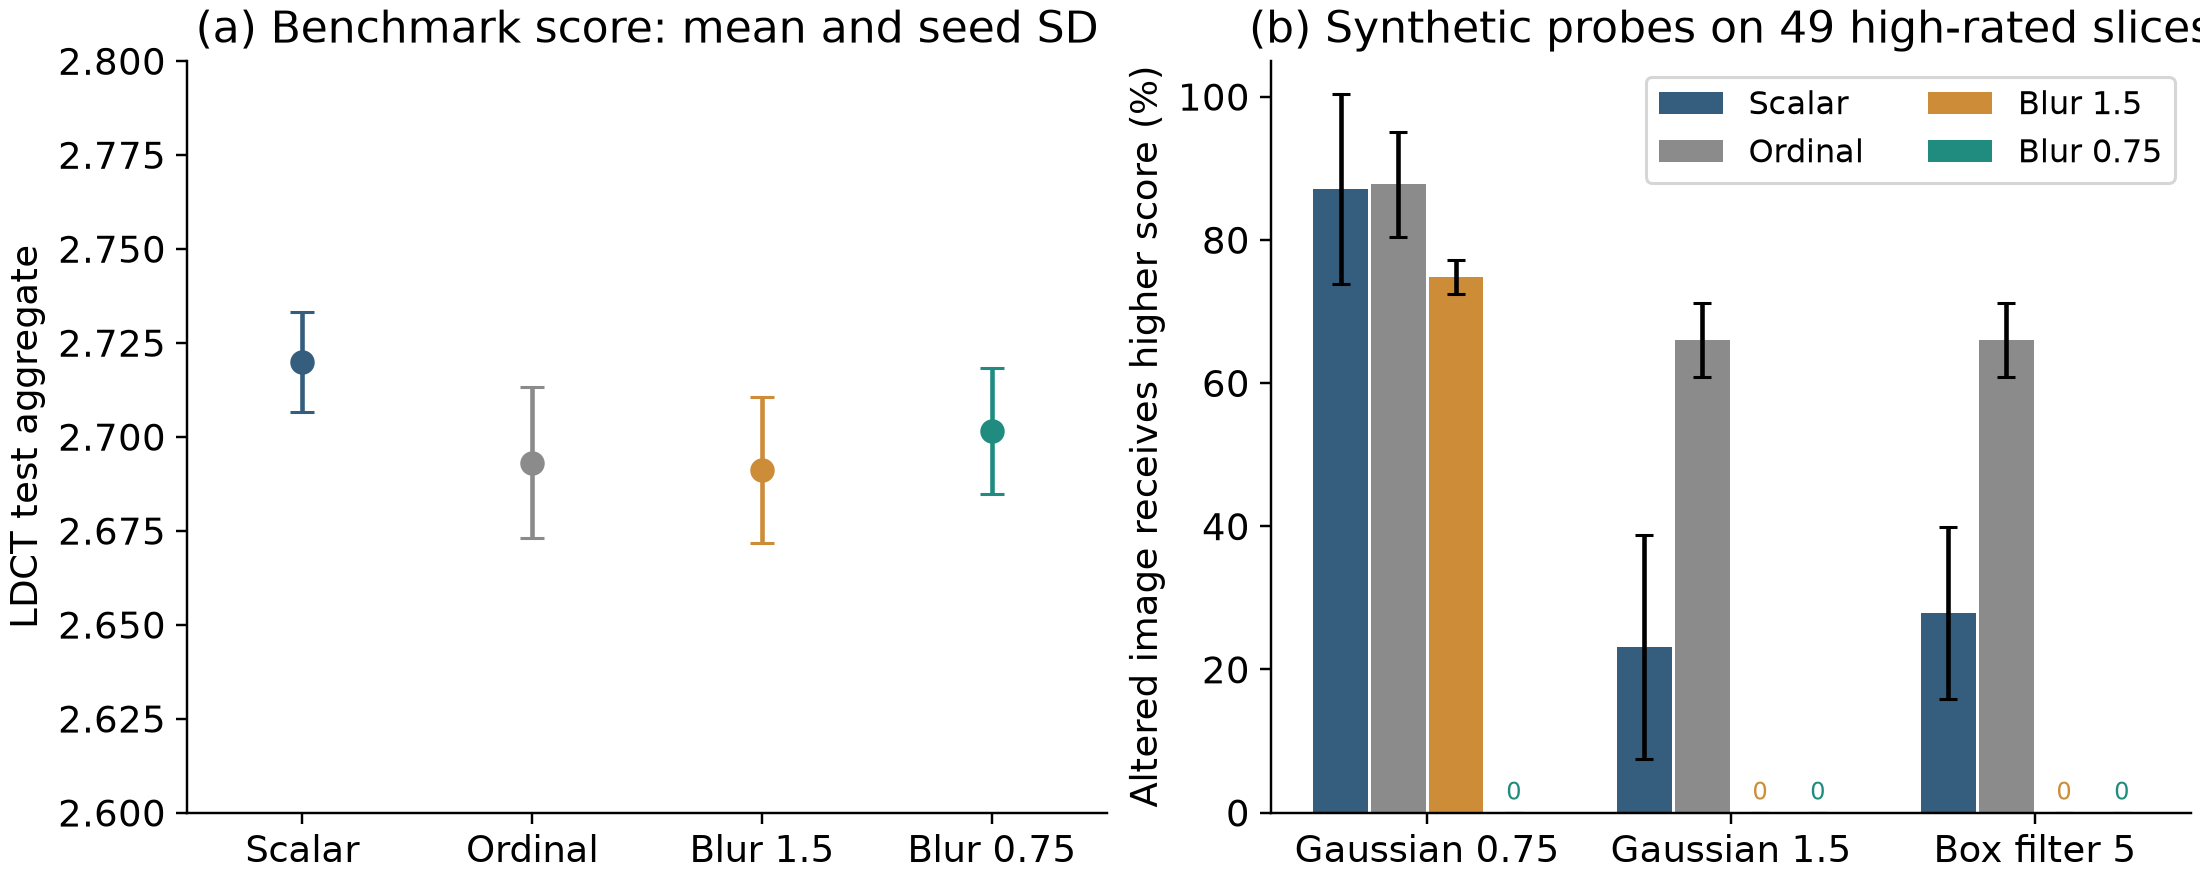
\includegraphics[width=\linewidth]{images/robustness_tradeoff.png}
\caption{Benchmark score and synthetic probe behavior. Left: mean and sample SD across three seeds. Right: fraction of 49 highly rated development images receiving a higher score after alteration, averaged across seeds. A higher score for a smoothed image is not automatically an error without transformed-image reader ratings.}\label{fig:tradeoff}
\end{figure}

\subsection{External expert agreement}
All 27 models were evaluated on all 1,666 annotated external images. The scalar baseline has signed Spearman correlation -0.142 and reader-pair agreement 42.5\%. The scalar conditional mild-blur control achieves 0.348 and 74.5\%, respectively, whereas its unconditional counterpart achieves -0.075 and 49.3\%. This supports a contribution from quality conditioning in this scalar mild-blur comparison, without demonstrating population-level generalization.

The original ordinal strong-blur constraint achieves correlation 0.426 and pair agreement 73.7\%, compared with -0.222 and 37.6\% without the constraint. However, the matched unconditional strong-blur arm achieves 0.391 and 72.8\%. The conditional-minus-unconditional intervals include zero for both endpoints (Table~\ref{tab:paired}); this arm does not isolate a reliable additional benefit from the quality gate.

The ordinal mild-blur arm has correlation -0.097 and pair agreement 48.4\%, despite eliminating score increases on the illustrated synthetic blur probes. ResNet-18 conditioning changes correlation from -0.603 to -0.470, but agreement remains poor (11.8\%). Synthetic constraint satisfaction therefore does not predict successful expert-rated transfer across heads and backbones.

Variation is substantial across training seeds and phantom anatomies (Table~\ref{tab:anatomy} and Figure~\ref{fig:external}). In particular, pooled gains do not establish stable pelvic performance. Paired source-slice intervals are descriptive summaries conditional on the two phantoms and the three fixed seeds; they do not capture uncertainty across patients, sites, physical phantoms or training-seed populations. Adaptive follow-up controls and multiple examined contrasts further limit confirmatory interpretation.

\begin{figure}[ht]\centering
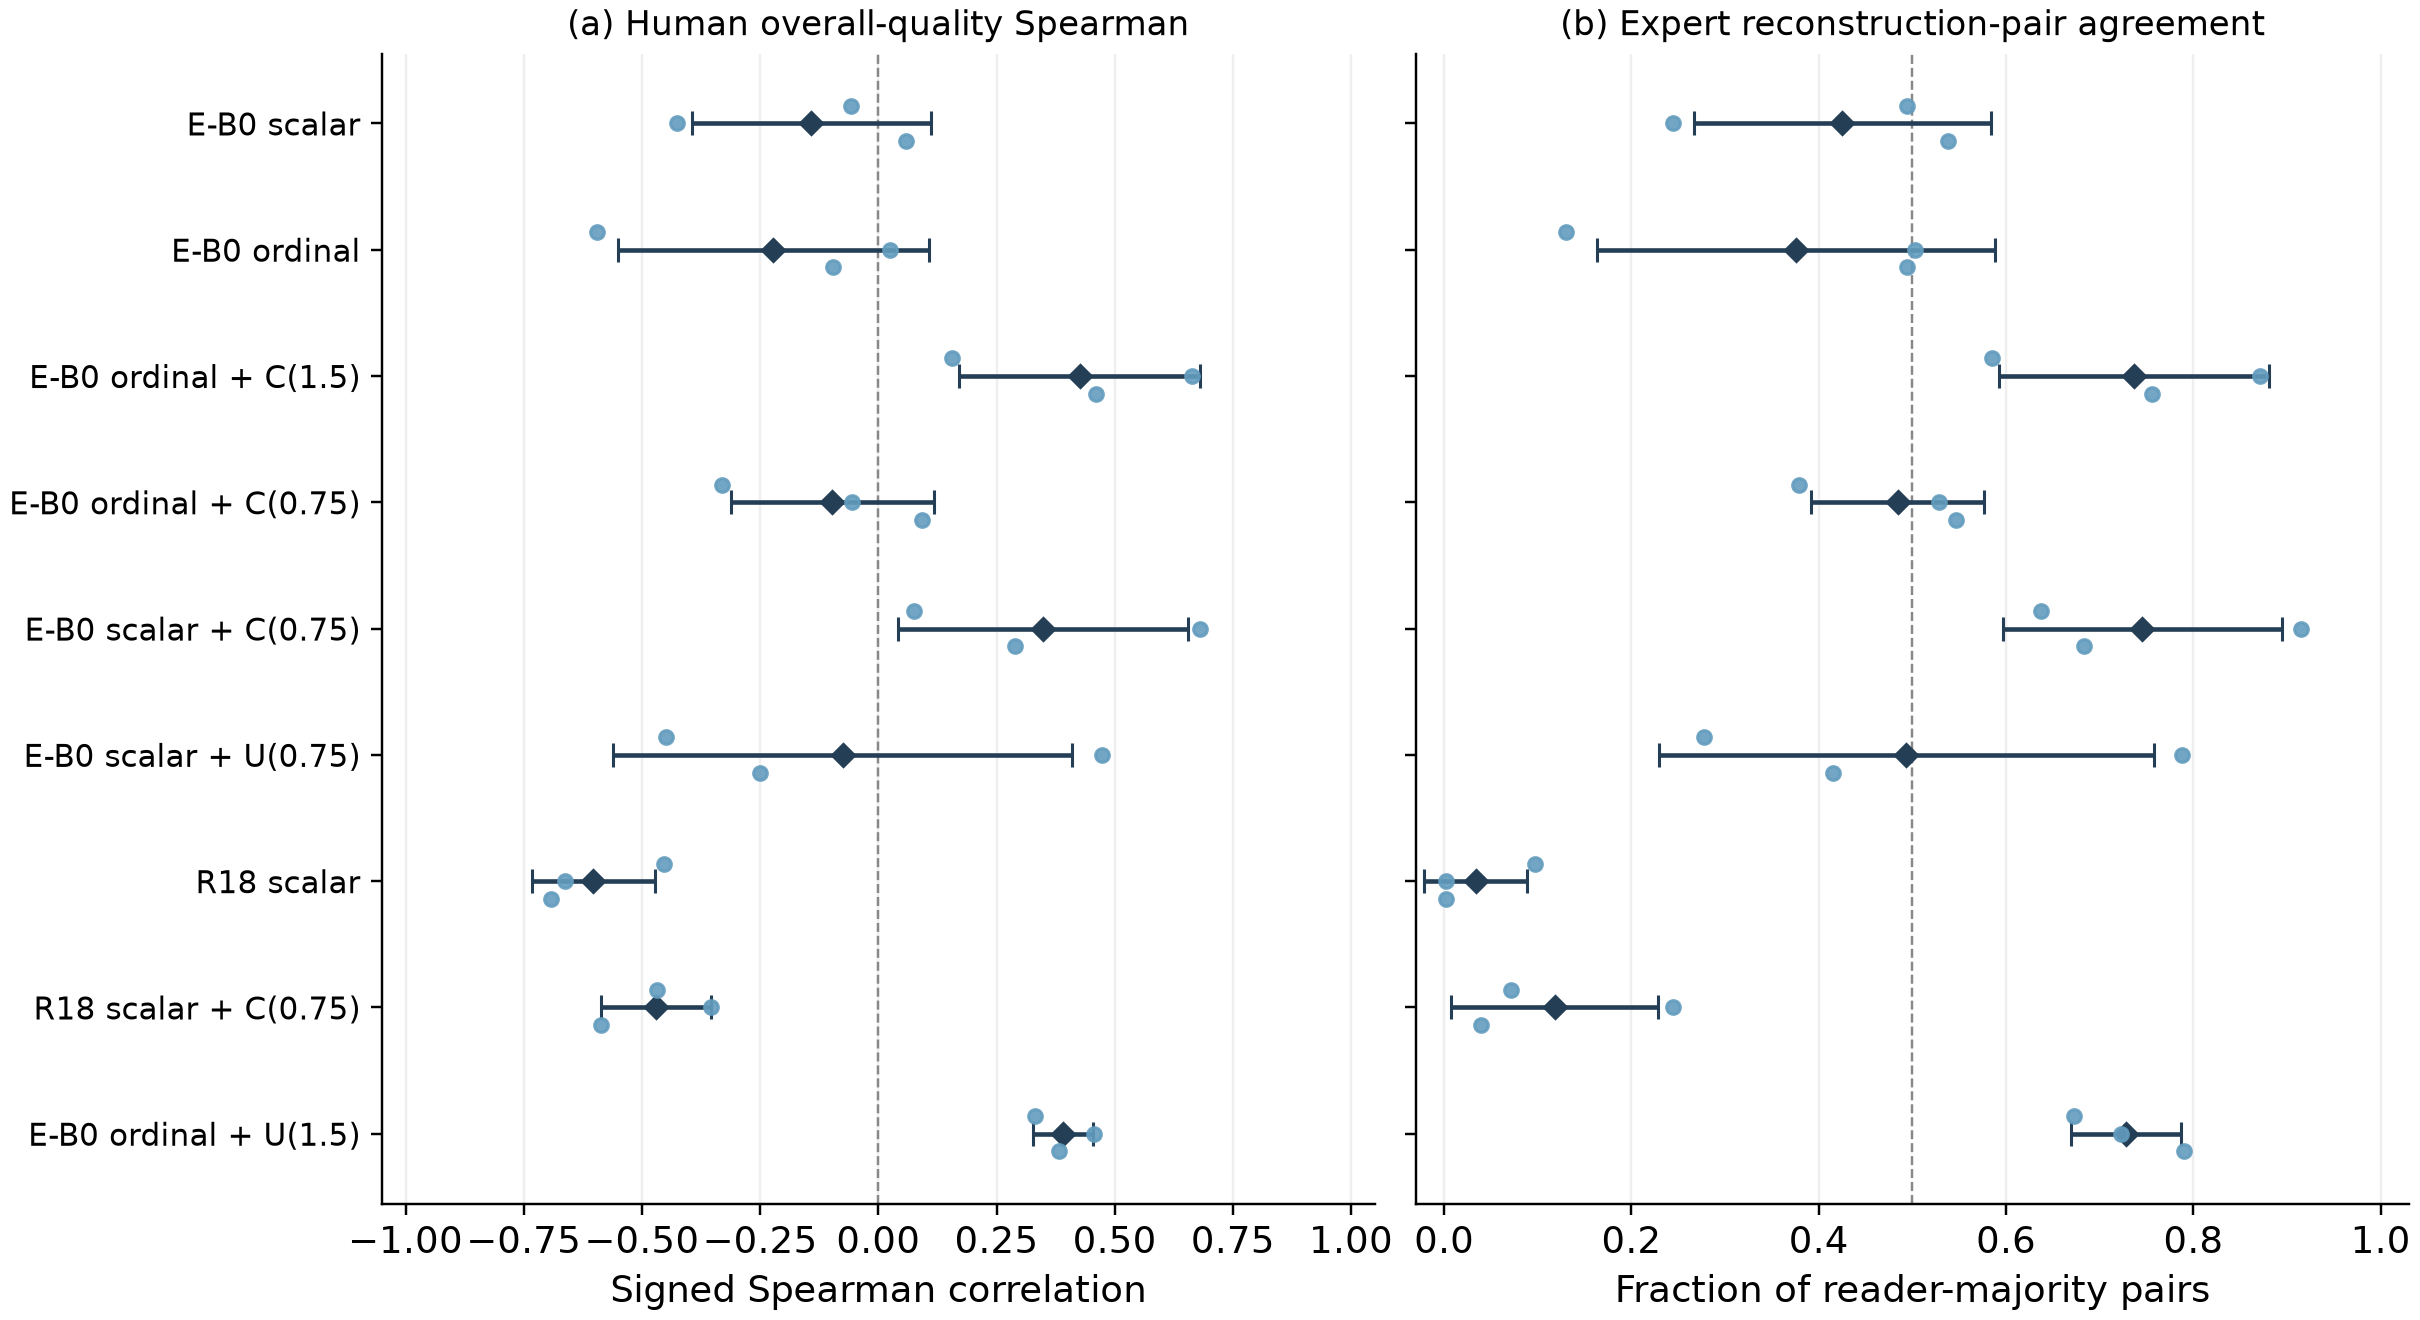
\includegraphics[width=\linewidth]{images/external_transfer.png}
\caption{External transfer for every declared arm. Diamonds and horizontal bars show means and sample SD across three fixed training seeds; small blue points show the individual seeds. E-B0 denotes EfficientNet-B0 and R18 denotes ResNet-18; C and U are conditional and universal blur ranking, with Gaussian $\sigma$ in parentheses. Dashed lines mark zero correlation and 50\% preference agreement. Error bars are not patient-population confidence intervals.}\label{fig:external}
\end{figure}
\section{Discussion}
The results distinguish three properties that are easily conflated: prediction of benchmark MOS, compliance with a synthetic degradation assumption, and agreement with independent expert judgments. A training constraint can improve the second property without improving the first or establishing the third. The scalar conditional control retains a similar observed benchmark aggregate while improving external expert agreement. In contrast, the ordinal mild-blur model satisfies the same illustrated synthetic probes yet transfers poorly. ResNet-18 also remains negatively correlated with the external ratings. The constraint can change a surrogate behavior without resolving the domain shift.

Conditioning on the original MOS limits the imposed rule on heavily degraded images, where smoothing may remove substantial noise. Its contribution is configuration-dependent: the scalar mild-blur control supports an advantage over universal ranking, whereas the strong ordinal comparison does not isolate an additional gate benefit. However, MOS $\geq3$ does not guarantee that all visible structure is diagnostically important, nor that additional mild smoothing is undesirable. The threshold narrows the assumption rather than validating it. External reconstruction comparisons are useful because their preference directions are supplied by experts rather than defined by the training transformation.

The compact architecture makes these controlled comparisons practical. Its use should not be confused with architectural novelty: EfficientNet-B0 is established, and high-resolution compact baselines already appear in recent CT-IQA work \cite{medsiglipcode}. Likewise, ordinal objectives and smoothing-bias analysis have prior art \cite{rps,measurement}. The contribution of this study must be judged from the controlled evidence on conditional training and transfer, including negative findings.

Benchmark results also need a consistent scoring protocol. Rounding predictions can change Kendall correlation through ties, and selecting the strongest test configuration can inflate an apparent result \cite{measurement}. We retain continuous predictions, disclose development adaptations and report all seeds. The observed absence of synthetic score increases should not be advertised as a calibrated safety guarantee or as validation for ranking arbitrary denoising algorithms.
\section{Limitations}
The LDCT development split uses inferred image groups because patient metadata are unavailable; patient overlap between development training and validation remains possible. The released test has prior exploratory use. Three training seeds quantify a limited source of variability, and the patient count in the benchmark is small. Any slice-group resampling remains conditional on inferred groups and cannot establish patient-level uncertainty.

The independent dataset comprises two phantoms and a different CT modality, anatomy mix, acquisition system and quality scale. It tests domain transfer rather than external patient-level clinical performance. Reconstruction preferences are correlated within source slices and acquisitions. Image counts therefore overstate the number of independent physical objects, and ordinary image-level correlation p-values are inappropriate as clinical significance evidence.

Two convolutional backbones and a small set of explicitly retained constraint controls are studied. Additional controls were added after initial external results, limiting confirmatory interpretation. The MOS threshold and ranking margin have not been broadly optimized, and a wider search could overfit the small development collection. No new radiologist assessment is available for the synthetic probes. A stronger clinical claim would require expert evaluation of relevant patient images and additional sites; the current results do not establish it.
\section{Conclusions}
Quality-conditioned blur ranking improves independent phantom reader agreement for a compact scalar CT-IQA model while retaining a similar observed benchmark aggregate. Matched controls show that the benefit depends on the prediction head, blur strength and backbone, and that satisfying synthetic blur constraints does not establish useful transfer. These exploratory findings support reporting benchmark accuracy, synthetic behavior and external expert agreement as separate properties. They establish neither state-of-the-art performance nor readiness for clinical deployment.
\section*{Declarations}
\textbf{Data and code availability.} LDCT challenge data and CBCT-IQ are provided by their respective sources \cite{challenge,cbctdata}. The accompanying repository contains evaluation code, fixed partitions, source snapshots, checksums and aggregate results. Original data and trained weights require their documented acquisition paths; neither is silently embedded in the code archive.

\textbf{Ethics.} This study uses previously released CT challenge data and public phantom data and collects no new reader ratings or patient scans. The authors must confirm the applicable institutional determination before submission; no new ethics approval or exemption is claimed here.

\textbf{Funding, competing interests and contributions.} These statements and the final author list require confirmation by the authors. OpenAI Codex assisted with code implementation, experiment orchestration, literature checking and manuscript drafting. Human author verification, interpretation and approval of the final manuscript remain required; an AI tool is not an author.

\clearpage
\appendix
\section{Complete synthetic probe summary}
G denotes Gaussian smoothing with the stated standard deviation, Box denotes box smoothing with the stated kernel width, and N denotes additive Gaussian noise with the stated standard deviation in normalized units. All original validation images remain included; the strata use only their original MOS. These are model response summaries, not error rates. Full score-change summaries are retained in the accompanying machine-readable results.
\begin{table}[ht]\centering\scriptsize
\caption{All development validation images ($n=210$): percentage receiving a higher score after each alteration, mean $\pm$ seed SD. These preferences have no transformed-image reader labels.}
\begin{tabular}{lrrrrrr}\toprule Model & G 0.75 & G 1.5 & G 2.5 & Box 5 & N .01 & N .03 \\ \midrule
Scalar & $97.0\pm3.1$ & $81.1\pm5.2$ & $69.0\pm7.7$ & $82.9\pm3.3$ & $4.4\pm2.4$ & $0.3\pm0.3$ \\
Ordinal & $97.1\pm1.7$ & $92.1\pm1.2$ & $80.5\pm7.3$ & $92.1\pm1.2$ & $3.2\pm2.3$ & $0.5\pm0.5$ \\
Ordinal + blur 1.5 & $94.1\pm0.5$ & $54.9\pm1.0$ & $53.7\pm1.7$ & $58.7\pm2.3$ & $3.7\pm2.7$ & $0.6\pm0.3$ \\
Ordinal + blur 0.75 & $58.6\pm3.8$ & $53.2\pm1.5$ & $59.5\pm5.9$ & $52.9\pm1.4$ & $4.6\pm3.8$ & $0.5\pm0.0$ \\
Scalar + conditional blur 0.75 & $56.3\pm1.7$ & $46.2\pm3.1$ & $48.1\pm4.2$ & $47.6\pm3.4$ & $3.8\pm2.2$ & $0.6\pm0.7$ \\
Scalar + unconditional blur 0.75 & $0.0\pm0.0$ & $3.8\pm2.1$ & $7.1\pm5.4$ & $1.7\pm2.6$ & $7.5\pm2.8$ & $0.3\pm0.5$ \\
ResNet-18 scalar & $100.0\pm0.0$ & $99.5\pm0.8$ & $96.0\pm5.3$ & $99.7\pm0.5$ & $2.4\pm1.7$ & $0.0\pm0.0$ \\
ResNet-18 + conditional blur 0.75 & $67.6\pm10.5$ & $34.8\pm12.4$ & $37.0\pm12.1$ & $38.7\pm9.4$ & $4.8\pm3.3$ & $0.0\pm0.0$ \\
Ordinal + unconditional blur 1.5 & $90.3\pm5.0$ & $0.2\pm0.3$ & $1.9\pm2.9$ & $4.0\pm1.0$ & $5.7\pm4.5$ & $0.8\pm0.5$ \\
\bottomrule\end{tabular}\end{table}
\begin{table}[ht]\centering\scriptsize
\caption{Original MOS at least 3 ($n=49$): percentage receiving a higher score after each alteration, mean $\pm$ seed SD. These preferences have no transformed-image reader labels.}
\begin{tabular}{lrrrrrr}\toprule Model & G 0.75 & G 1.5 & G 2.5 & Box 5 & N .01 & N .03 \\ \midrule
Scalar & $87.1\pm13.3$ & $23.1\pm15.6$ & $6.1\pm8.9$ & $27.9\pm12.0$ & $0.0\pm0.0$ & $0.0\pm0.0$ \\
Ordinal & $87.8\pm7.4$ & $66.0\pm5.1$ & $27.9\pm21.6$ & $66.0\pm5.1$ & $0.0\pm0.0$ & $0.0\pm0.0$ \\
Ordinal + blur 1.5 & $74.8\pm2.4$ & $0.0\pm0.0$ & $0.0\pm0.0$ & $0.0\pm0.0$ & $0.0\pm0.0$ & $0.0\pm0.0$ \\
Ordinal + blur 0.75 & $0.0\pm0.0$ & $0.0\pm0.0$ & $0.0\pm0.0$ & $0.0\pm0.0$ & $0.0\pm0.0$ & $0.0\pm0.0$ \\
Scalar + conditional blur 0.75 & $0.0\pm0.0$ & $0.0\pm0.0$ & $0.0\pm0.0$ & $0.0\pm0.0$ & $0.0\pm0.0$ & $0.0\pm0.0$ \\
Scalar + unconditional blur 0.75 & $0.0\pm0.0$ & $0.0\pm0.0$ & $0.0\pm0.0$ & $0.0\pm0.0$ & $0.0\pm0.0$ & $0.0\pm0.0$ \\
ResNet-18 scalar & $100.0\pm0.0$ & $98.0\pm3.5$ & $83.0\pm22.8$ & $98.6\pm2.4$ & $0.0\pm0.0$ & $0.0\pm0.0$ \\
ResNet-18 + conditional blur 0.75 & $11.6\pm11.2$ & $0.0\pm0.0$ & $0.0\pm0.0$ & $0.0\pm0.0$ & $0.0\pm0.0$ & $0.0\pm0.0$ \\
Ordinal + unconditional blur 1.5 & $72.8\pm14.8$ & $0.0\pm0.0$ & $0.0\pm0.0$ & $0.0\pm0.0$ & $0.0\pm0.0$ & $0.0\pm0.0$ \\
\bottomrule\end{tabular}\end{table}
\begin{table}[ht]\centering\scriptsize
\caption{Original MOS at most 1 ($n=49$): percentage receiving a higher score after each alteration, mean $\pm$ seed SD. These preferences have no transformed-image reader labels.}
\begin{tabular}{lrrrrrr}\toprule Model & G 0.75 & G 1.5 & G 2.5 & Box 5 & N .01 & N .03 \\ \midrule
Scalar & $100.0\pm0.0$ & $100.0\pm0.0$ & $100.0\pm0.0$ & $100.0\pm0.0$ & $12.9\pm5.9$ & $1.4\pm1.2$ \\
Ordinal & $100.0\pm0.0$ & $100.0\pm0.0$ & $100.0\pm0.0$ & $100.0\pm0.0$ & $11.6\pm8.5$ & $2.0\pm2.0$ \\
Ordinal + blur 1.5 & $100.0\pm0.0$ & $100.0\pm0.0$ & $100.0\pm0.0$ & $100.0\pm0.0$ & $12.2\pm9.4$ & $2.7\pm1.2$ \\
Ordinal + blur 0.75 & $100.0\pm0.0$ & $100.0\pm0.0$ & $100.0\pm0.0$ & $100.0\pm0.0$ & $14.3\pm11.4$ & $2.0\pm0.0$ \\
Scalar + conditional blur 0.75 & $100.0\pm0.0$ & $100.0\pm0.0$ & $100.0\pm0.0$ & $100.0\pm0.0$ & $10.2\pm3.5$ & $2.7\pm3.1$ \\
Scalar + unconditional blur 0.75 & $0.0\pm0.0$ & $16.3\pm8.9$ & $28.6\pm19.5$ & $7.5\pm11.2$ & $16.3\pm5.4$ & $1.4\pm2.4$ \\
ResNet-18 scalar & $100.0\pm0.0$ & $100.0\pm0.0$ & $100.0\pm0.0$ & $100.0\pm0.0$ & $4.8\pm5.1$ & $0.0\pm0.0$ \\
ResNet-18 + conditional blur 0.75 & $97.3\pm4.7$ & $88.4\pm10.1$ & $88.4\pm11.2$ & $91.2\pm7.7$ & $7.5\pm6.6$ & $0.0\pm0.0$ \\
Ordinal + unconditional blur 1.5 & $98.0\pm3.5$ & $0.7\pm1.2$ & $7.5\pm11.2$ & $15.0\pm3.1$ & $17.0\pm15.6$ & $3.4\pm2.4$ \\
\bottomrule\end{tabular}\end{table}

\clearpage
\section{Paired external comparisons}
\begin{table}[ht]\centering\scriptsize
\caption{Paired differences with 95\% source-slice bootstrap percentile intervals within the two fixed phantoms, averaging three fixed seeds. C restricts the blur constraint to training MOS $\geq3$; U applies it universally. These intervals do not quantify patient/site or training-seed population uncertainty.}
\begin{tabular}{lrr}\toprule Contrast & $\Delta$ Spearman [interval] & $\Delta$ pair agreement [interval] \\ \midrule
Ordinal C1.5 -- ordinal & $+0.648\;[+0.627,+0.670]$ & $+0.361\;[+0.343,+0.380]$ \\
Ordinal C0.75 -- ordinal & $+0.125\;[+0.039,+0.209]$ & $+0.109\;[+0.067,+0.150]$ \\
Ordinal C1.5 -- scalar & $+0.568\;[+0.534,+0.605]$ & $+0.312\;[+0.288,+0.336]$ \\
Ordinal C0.75 -- scalar & $+0.044\;[-0.024,+0.116]$ & $+0.059\;[+0.013,+0.107]$ \\
Scalar C0.75 -- scalar & $+0.490\;[+0.434,+0.554]$ & $+0.320\;[+0.275,+0.366]$ \\
Scalar C0.75 -- scalar U0.75 & $+0.424\;[+0.403,+0.445]$ & $+0.252\;[+0.240,+0.263]$ \\
ResNet C0.75 -- ResNet & $+0.133\;[+0.112,+0.151]$ & $+0.084\;[+0.072,+0.097]$ \\
Ordinal C1.5 -- ordinal U1.5 & $+0.036\;[-0.001,+0.070]$ & $+0.009\;[-0.011,+0.030]$ \\
\bottomrule\end{tabular}\label{tab:paired}\end{table}

\begin{thebibliography}{99}
\bibitem{challenge} W. Lee et al. Low-dose computed tomography perceptual image quality assessment. \emph{Medical Image Analysis} 99 (2025), 103343. \url{https://doi.org/10.1016/j.media.2024.103343}.
\bibitem{winner} A. Galdran. LDCT-IQA challenge winning implementation. \url{https://github.com/agaldran/ldct_iqa}. Accessed 25 November 2026.
\bibitem{rps} A. Galdran. Performance Metrics for Probabilistic Ordinal Classifiers. \url{https://arxiv.org/abs/2309.08701}.
\bibitem{medsiglip} T. Demiroglu et al. Prompt-Conditioned FiLM and Multi-Scale Fusion on MedSigLIP for Low-Dose CT Quality Assessment. Preprint (2025). \url{https://arxiv.org/abs/2511.12256}.
\bibitem{clinreadnet} X. Xiao et al. ClinReadNet: A clinical reading-inspired network for low-dose abdominal CT image quality assessment. \emph{Neural Networks} 197 (2026), 108535. \url{https://doi.org/10.1016/j.neunet.2025.108535}.
\bibitem{medsiglipcode} MedSigLIP-LDCT-IQA author implementation and updated comparisons. \url{https://github.com/itu-biai/medsiglip-ldct-iqa}. Accessed 25 November 2026. Repository results differ from the initial preprint.
\bibitem{measurement} K. Basim et al. Measurement-Aware Multimodal LLM for No-Reference Low-Dose CT Quality Assessment. Preprint (2026). \url{https://arxiv.org/abs/2611.08754}.
\bibitem{cbctpaper} S. Hatamikia et al. CBCT-IQ: A Publicly Available Annotated Cone-Beam CT Dataset for Image Quality Assessment and Benchmarking. Preprint (2026). \url{https://arxiv.org/abs/2607.29253}.
\bibitem{cbctdata} S. Hatamikia et al. CBCT-IQ dataset, version 1.0 (2026). \url{https://doi.org/10.5281/zenodo.20124496}. CC BY 4.0.
\bibitem{rankiqa} X. Liu, J. van de Weijer and A. D. Bagdanov. RankIQA: Learning From Rankings for No-Reference Image Quality Assessment. ICCV (2017), 1040--1049. \url{https://openaccess.thecvf.com/content_iccv_2017/html/Liu_RankIQA_Learning_From_ICCV_2017_paper.html}.
\bibitem{distortionct} Q. Bourbon et al. Distortion-Guided Learning for Opinion-Unaware No-Reference Image Quality Assessment in Low Dose CT. ISBI (2026). \url{https://doi.org/10.1109/ISBI61048.2026.11515364}.
\bibitem{efficientnet} M. Tan and Q. V. Le. EfficientNet: Rethinking Model Scaling for Convolutional Neural Networks. ICML (2019). \url{https://arxiv.org/abs/1905.11946}.
\end{thebibliography}
\end{document}
